\documentclass[a4paper]{article}
\usepackage{amsfonts}
\usepackage{amsmath}
\usepackage{amssymb}
\usepackage{graphicx}     

\begin{document}
  
\noindent \large Auteur: Thomas \\
\noindent \large Studierichting: Informatica\\
\noindent \large Oefeningenreeks 3H nr. 8.2\\

\medskip

\normalsize

$r = 2 \cos(2\theta)$ \\

Periode = $\pi$ , beperkt domein: $[0,\pi]$ \\

nulpunten: $2\cos(2\theta) = 0 \Leftrightarrow \cos(2\theta) = 0 \Leftrightarrow \theta = \dfrac{\pi}{4}, \dfrac{3\pi}{4}$ \\

$r' = 2(-\sin 2\theta) \cdot 2 = 4 (-\sin 2\theta)$ \\

nulpunten: $4(-\sin 2\theta) = 0 \Leftrightarrow \theta = 0, \dfrac{\pi}{2}, \pi$ \\

$\begin{array}{r | c c c c c c c c c}
\theta & 0 & & \dfrac{\pi}{4} & & \dfrac{\pi}{2} & & \dfrac{3\pi}{4} & & \pi\\ \hline
r(\theta) & + & + & 0 & - & - & - & 0 & + & + \\
r'(\theta) & 0 & - & - & - & 0 & + & + & + & 0 \\ \hline
r(\theta) & M(2) & \searrow & \searrow & \searrow & m(-2) & \nearrow & \nearrow & \nearrow & M(2) \\
\end{array}$ \\

\begin{figure}[h]
\centering
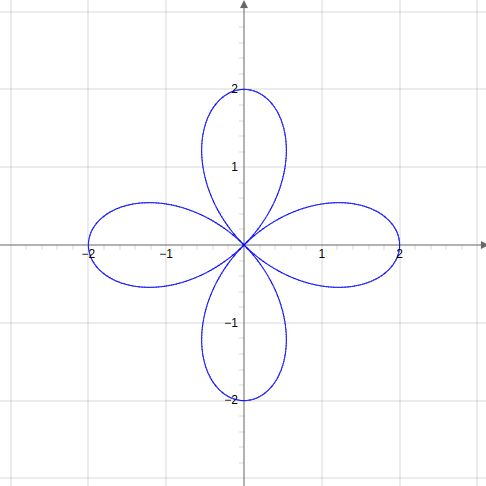
\includegraphics[width = 7cm]{3H-8.2-thomas.eertmans.INF.png}
\end{figure}



\begin{thebibliography}{999}
%\bibitem{a} Referentie
\end{thebibliography}
\end{document} 
